\documentclass[a4paper,12pt]{article}

% Paquetes básicos
\usepackage[utf8]{inputenc}
\usepackage[T1]{fontenc}
\usepackage[spanish]{babel}
\usepackage{graphicx}
\usepackage{xcolor}
\usepackage{lipsum}
\usepackage{geometry}
\geometry{top=3cm, bottom=3cm, left=2.5cm, right=2.5cm}


% Paquetes para diseño
\usepackage{titlesec}
\usepackage{fancyhdr}
\usepackage{amsmath}
\usepackage{amssymb}
\usepackage{hyperref}
\usepackage{float}
\usepackage{eurosym}
\usepackage{tcolorbox}

% Paquetes para el entorno lstlisting
\usepackage{listings}
\usepackage{inconsolata}

% Paquete para fondo
\usepackage{background}

% Configuración de lstlisting
\lstset{
    language=Python,
    basicstyle=\ttfamily\small,
    keywordstyle=\color{blue}\bfseries,
    stringstyle=\color{teal},
    commentstyle=\color{gray}\itshape,
    numbers=left,
    numberstyle=\tiny\color{gray},
    backgroundcolor=\color{black!5},
    frame=single,
    rulecolor=\color{black!50},
    breaklines=true,
    captionpos=b,
    showstringspaces=false
}

\newcommand{\fec}{31/12/}
\newcommand{\AIM}{681 Amortización del inmovilizado material }
\newcommand{\AAMAQ}{2813 Amortización acumulada de maquinaria }
\newcommand{\valorrecuperable}{Valor recuperable = max\{valor neto realizable, valor en uso\} =}
\newcommand{\PDI}{691 Pérdidas por deterioro de inmovilizado material}
\newcommand{\DVM}{2913 Deterioro del valor de la maquinaria }
\newcommand{\RDIM}{791 Reversión deterioro inmovilizado material}
\newcommand{\VC}{Valor contable = }
\newcommand{\PPIM}{671 Pérdidas procedentes del inmovilizado material}
\newcommand{\bancos}{572 Bancos cuenta corriente}
\newcommand{\cuotaamort}{Cuota de amortización = }
\newcommand{\enajenacion}{543 Créditos a corto plazo por enajenación del inmovilizado}
\newcommand{\benefIM}{771 Beneficios procedentes del inmovilizado material}
\usepackage{amsmath}
\newcommand{\myequation}[2]{\ensuremath{\frac{#1}{#2}}}
\newcommand{\flechita}{$\rightarrow$}
%comando de tcolorbox
\newcommand{\mytcolorbox}[1]{
    \begin{tcolorbox}[colback=blue!5!white, colframe=blue!75!black, title=NOTA]
        #1
    \end{tcolorbox}
}





% Configuración de título
\titleformat{\section}{\normalfont\Large\bfseries}{\thesection}{1em}{}

% Información del documento
\title{
    \vspace{-2cm}
    
\includegraphics[width=0.3\textwidth]{images/fccee.jpg} \\ % Cambia el logo si es necesario
    \LARGE Ingeniería Informática + ADE\\
    \large Universidad de Granada (UGR)\\[1cm]
}
\author{\textbf{Autor:} Ismael Sallami Moreno}
\date{\textbf{Asignatura:} Ejercicios Propuestos Resueltos Tema 4}

% Configuración del fondo
\backgroundsetup{
    scale=1,
    color=black,
    opacity=0.2,
    angle=0,
    position=current page.south,
    vshift=0pt,
    hshift=0pt,
    contents={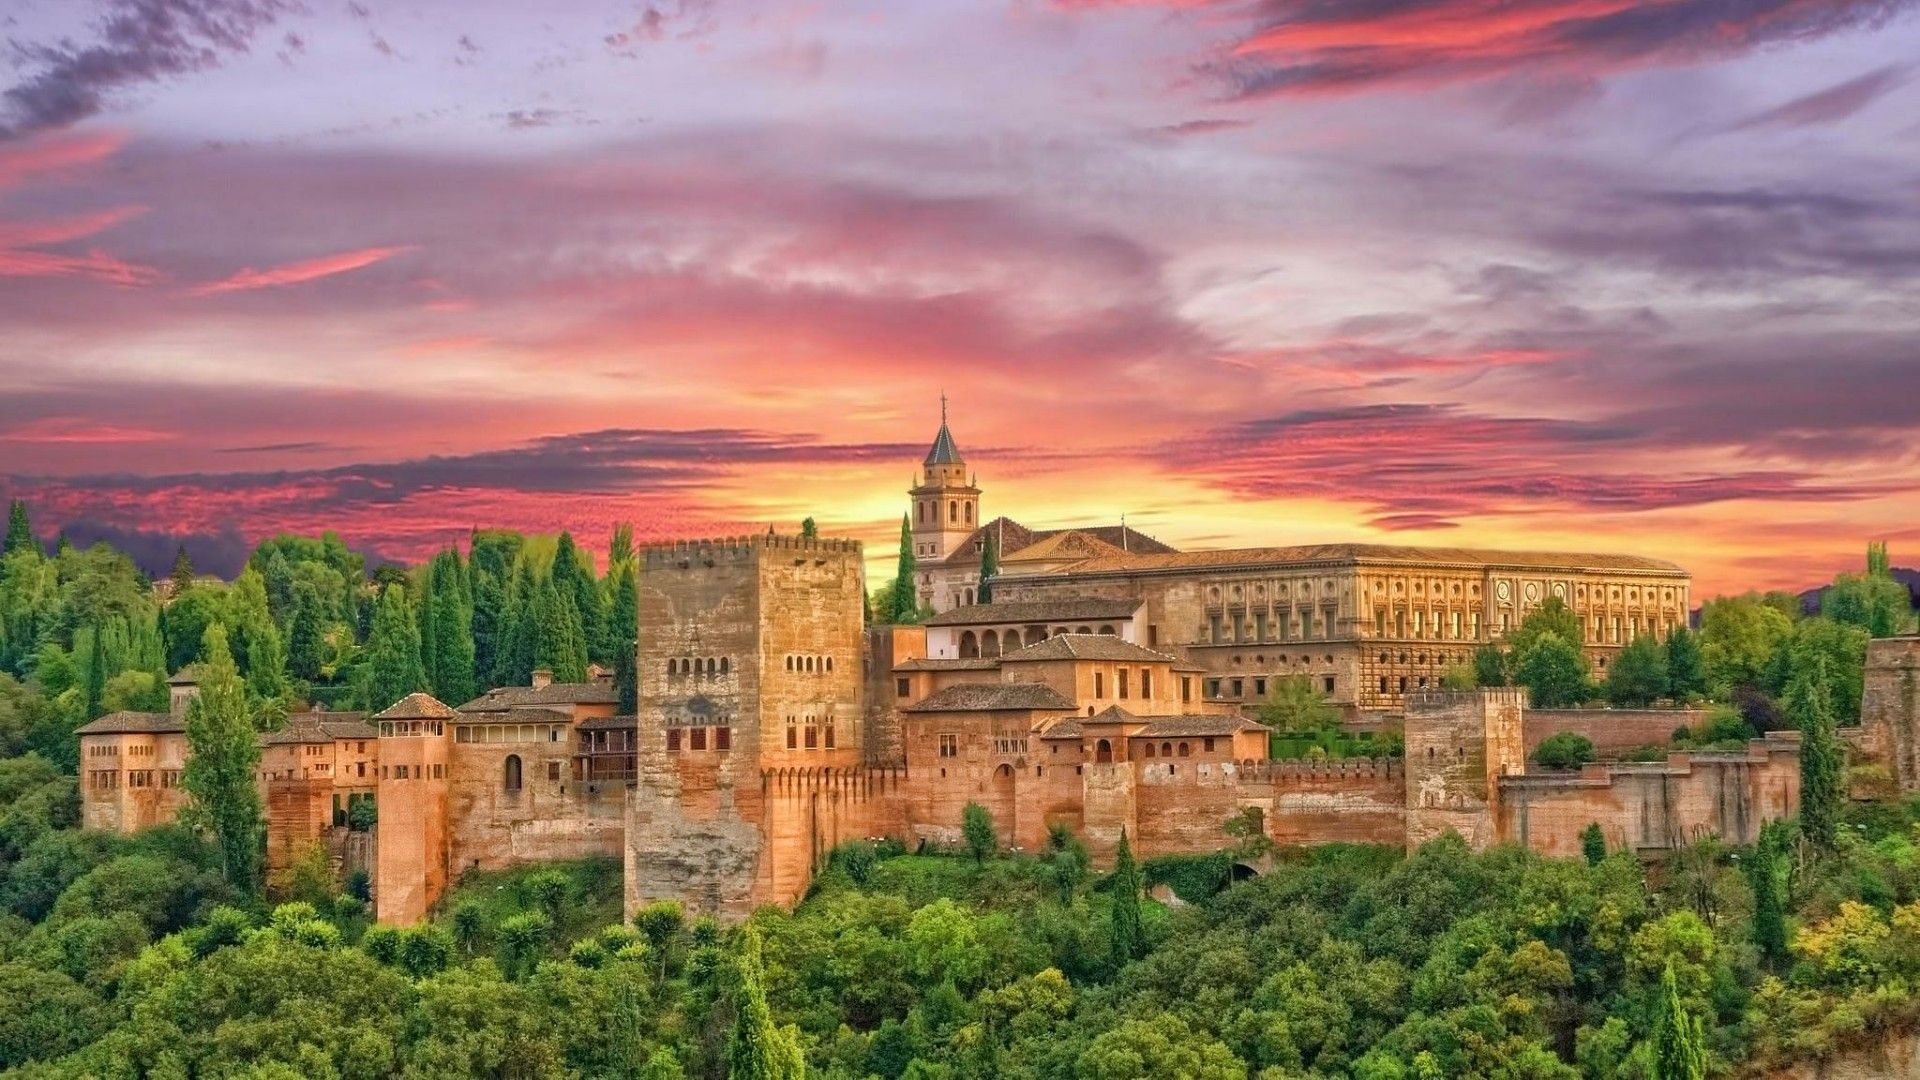
\includegraphics[width=\paperwidth,height=\paperheight,keepaspectratio]{images/granada.jpg}}
}
% Cambiar la fuente a Palatino
\usepackage{mathpazo}

% Inicio del documento
\begin{document}

% Portada
\maketitle
\thispagestyle{empty}

\begin{center}
    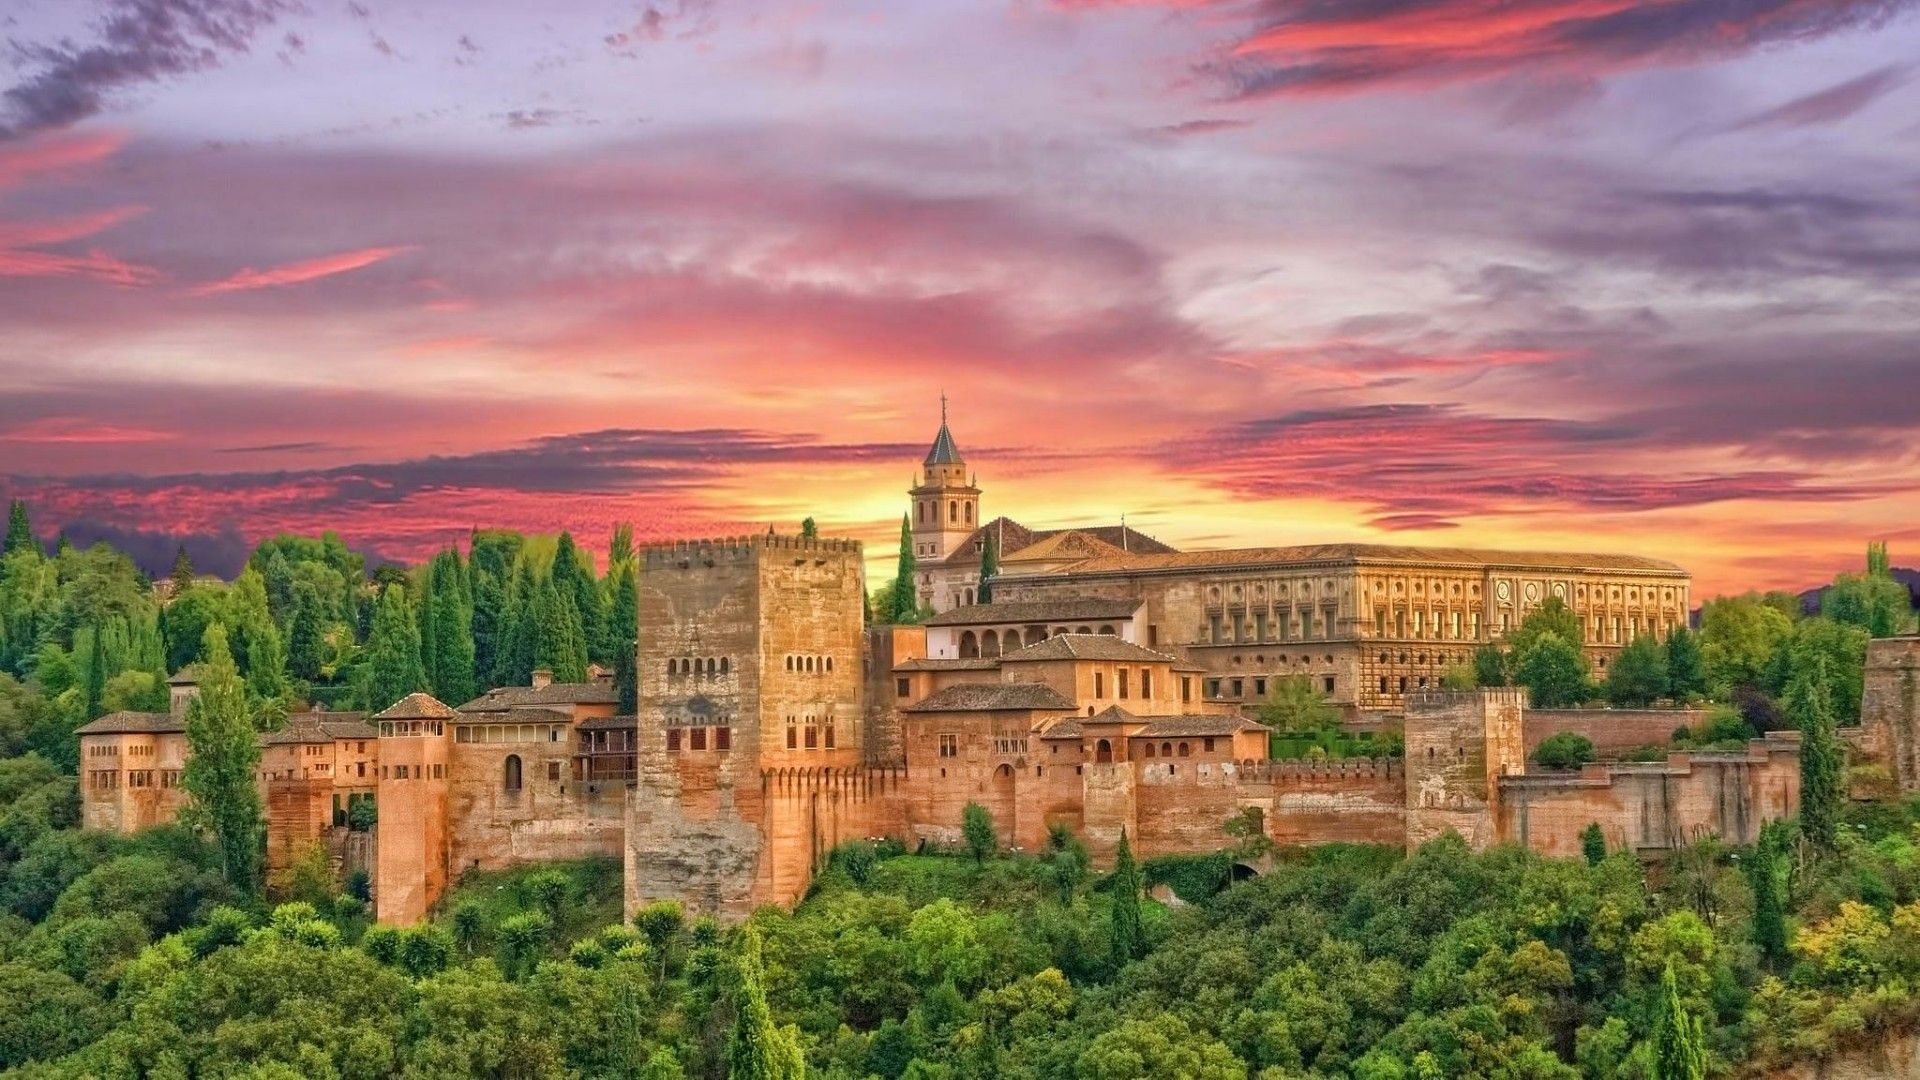
\includegraphics[width=\textwidth,height=0.4\textheight,keepaspectratio]{images/granada.jpg} \\ % Añade tu imagen de fondo
    \vfill
\end{center}

\newpage

% Índice (opcional)
\tableofcontents
\newpage

\textbf{NOTA:} Los enunciados se encuentran en el libro.

\section{Ejercicio Propuesto 1}
\subsection*{APARTADO 1}
\begin{itemize}
    \item Nos dan el balance de saldos
    \item Se compran 20 unidades a 3 \euro
    \item descuento del 1 \%
    \item se paga mediante cheque los transportes que ascienden a 10 \euro
    \item Iva del 21\%
\end{itemize}

\begin{table}[H]
    \centering
    \begin{tabular}{|p{3cm}|p{6cm}|p{3cm}|}
    \hline
    \textbf{DEBE} & \textbf{Compra de mercaderías} & \textbf{HABER} \\
    \hline
    $20 * 3* 0,99 + 10 = 69,4 $& (600) Compra de mercaderías & \\
    \hline
    $0,21*69,4 = 14,574$& (472) IVA H.P soportado & \\
    \hline
    & 400 Proveedores & $59,4 * 1,21 = 71,874$\\
    \hline
    & 572 Bancos &$10 * 1,21 = 12,1$ \\
    \hline
    % & & \\
    % \hline
    \end{tabular}
    \end{table}
\subsection*{APARTADO 2}

\begin{itemize}
    \item paga la nómina en diciembre
    \item deja pendiente de pago 100 \euro 
    \item aplicar anticipo total existente
    \item sueldo bruto de 1600 \euro
    \item cuota obrera es 480 \euro
    \item cuota patronal 360 \euro
\end{itemize}

\begin{table}[H]
    \centering
    \begin{tabular}{|p{3cm}|p{6cm}|p{3cm}|}
    \hline
    \textbf{DEBE} & \textbf{nómina} & \textbf{HABER} \\
    \hline
    1600 & 640 sueldo y salarios& \\
    \hline
    360 & 642 SS a cargo de la empresa& \\
    \hline
    & 476 org seg soc acreedora & $360 + 480$ \\
    \hline
    & 460 anticipos de remuneraciones& 200\\
    \hline
    &4751 hp retenciones y pagos & 320\\
    \hline
    & 465 remuneraciones pendientes de pago & 100\\
    \hline
    & 572 bancos & 500\\
    \hline
    \end{tabular}
    \end{table}

    \subsection*{APARTADO 3}
    \begin{itemize}
        \item La empresa no vende mercaderías durante el ejercicio contable
        \item a 31/12/2021 se valoran las mercaderías de la empresa a 4 \euro
        \item costes de comercialización de 10,5 \euro
        \item contrató y pagó por adelantado el 1 de diciembre la prima de seguros, debemos de contabilizar lo que no se ha consumido en este ejercicio
    \end{itemize}

    \begin{table}[H]
        \centering
        \begin{tabular}{|p{3cm}|p{6cm}|p{3cm}|}
        \hline
        \textbf{DEBE} & \textbf{Prima de seguros} & \textbf{HABER} \\
        \hline
        $1100 = 1200 - 1200/12 * 1 $ & 480 gastos anticipados & \\
        \hline
        &625 Prima de Seguros & 1100 \\
        \hline
        
        \end{tabular}
        \end{table}
    
    \subsection*{APARTADO 4}
    \begin{itemize}
        \item el 1 de dicembre la empresa alquiló un un local por 1800 \euro
        \item contrato con duración de 6 meses
    \end{itemize}

    \begin{table}[H]
        \centering
        \begin{tabular}{|p{3cm}|p{6cm}|p{3cm}|}
        \hline
        \textbf{DEBE} & \textbf{Ingresos por arrendamiento} & \textbf{HABER} \\
        \hline
        $ 1800/6 * 1 = 300 ; 1800-300 = 1500 $ & 752 ingresos por arrendamientos & \\
        \hline
        & 485 ing anticipados & 1500 \\
        \hline
        
        \end{tabular}
        \end{table}

    \subsection*{APARTADO 5}
    \begin{itemize}
        \item Hacer el resultado del Ejercicio
    \end{itemize}

    \begin{table}[H]
        \centering
        \begin{tabular}{|p{3cm}|p{6cm}|p{3cm}|}
        \hline
        \textbf{DEBE} & \textbf{operaciones en relación a las mercaderías a 31/12/2021} & \textbf{HABER} \\
        \hline
        69,4 & 300 mercaderías& \\
        \hline
        & 610 var de existencias & 69,4\\
        \hline
        
        \end{tabular}
        \end{table}

        \begin{table}[H]
            \centering
            \begin{tabular}{|p{3cm}|p{6cm}|p{3cm}|}
            \hline
            \textbf{DEBE} & \textbf{Cálculo del resultado: Gastos} & \textbf{HABER} \\
            \hline
            2209,4 & 129 rdo del ejercicio & \\
            \hline
            & 600 compra mercaderías & 69,4\\
            \hline
            & 640 sueldos y salarios & 1600 \\
            \hline
            & 642 ss a cargo de la empresa & 360\\
            \hline
            & 625 prima de seguros& $1200/12  * 1 = 100$\\
            \hline
            & 624 transportes & 80 \\
            \hline
            \end{tabular}
            \end{table}

            \begin{table}[H]
                \centering
                \begin{tabular}{|p{3cm}|p{6cm}|p{3cm}|}
                \hline
                \textbf{DEBE} & \textbf{Cálculo del resultado: Ingresos} & \textbf{HABER} \\
                \hline
                300 & 752 Ing Arrendamientos & \\
                \hline
                69,4& 610 var existencias& \\
                \hline
                & 129 rdo del ejercicio & 369,4 \\
                \hline
                \end{tabular}
                \end{table}
    
                \subsubsection*{Resultado del ejercicio:}
                Podemos ver como el saldo de la cuenta 129 Resultado del ejercicio al final del período es:
                \begin{equation}
                    469,4 - 2209,4 = -1740
                \end{equation}
                \textit{Este resultado indica que el saldo de la cuenta 129 Resultado del ejercicio al final del período es negativo, lo que significa que la empresa ha obtenido pérdidas de 1740 euros.}

\section{Ejercicio Propuesto 2}
\subsection*{Datos}
\begin{itemize}
    \item 1 de abril de 2020 compra a un proveedor mercancías por valor de 11.500 rublos
    \item descuento de 1500 rublos
    \item gastos de transportes, seguro y aduana 500 rublos
    \item pagados por transferencia bancaria
    \item el pago se realiza en 18 meses
    \item intereses aplazamiento del 4 \%
    \item tipo de cambio a la fecha de la compra es de 1 rublo = 2,5 euros
    \item al cierre el tipo de cambio es de 1 rublo = 2,6 euros
    \item el dia del vencimiento es 2,4 euros = 1 rublo
\end{itemize}

\begin{table}[H]
    \centering
    \begin{tabular}{|p{3cm}|p{6cm}|p{3cm}|}
    \hline
    \textbf{DEBE} & \textbf{compra de mercaderias a 1/4/2020} & \textbf{HABER} \\
    \hline
    26.250& 600 Compra de mercaderias& \\
    \hline
    & 4004 Proveedores en moneda extranjera& 10.000 rublos a 2,5 euros/rublo = 25.000\\
    \hline
    & 572 Bancos & 500 * 2,5 = 1250\\
    \hline
    \end{tabular}
\end{table}
\begin{itemize}
    \item Cambio en el tipo de cambio de la moneda, que pasa de 2,5 euro/rublo a 2,6 euro/rublo.
    \item Por lo que debemos de dotar las diferencias negativas de cambio ya que le vamos a pagar más al proveedor al valorarse el rublo.
    \item El valor de la deuda pasa de 10.000 * 2,5 a 10.000 * 2,6 = 26.000, siendo la diferencia de: 1.000 euros.
\end{itemize}

\begin{table}[H]
    \centering
    \begin{tabular}{|p{3cm}|p{6cm}|p{3cm}|}
    \hline
    \textbf{DEBE} & \textbf{a \fec2020 operaciones relacionadas con la deuda del proveedor} & \textbf{HABER} \\
    \hline
    & 4004 Proveedores en moneda extranjera& 1000\\
    \hline
    1000& 668 Diferencias negativas de Cambio& \\
    \hline
    \end{tabular}
\end{table}

\begin{itemize}
    \item El cálculo de los intereses es:
    \begin{itemize}
        \item 9 meses
        \item 4 \% de intereses
        \item $10000 \textbf{ rublos } * 1,04^{\frac{9}{12}} - 10000 = 298,52$
        \item Pasamos a euros con el tipo de cambio de 2,6 euros/rublo, por lo que 298,52 * 2,6 = 776,17
    \end{itemize}
\end{itemize}
\begin{tcolorbox}[colback=red!5!white,colframe=yellow!75!black, title={Nota}]
    El tipo de cambio también se calcula tomando como montante el valor en la moneda del extranjero.
\end{tcolorbox}

\begin{table}[H]
    \centering
    \begin{tabular}{|p{3cm}|p{6cm}|p{3cm}|}
    \hline
    \textbf{DEBE} & \textbf{a \fec2020 devengo de los intereses por aplazamiento de pago a los prooveedores} & \textbf{HABER} \\
    \hline
    776,17& 662 Intereses de deudas& \\
    \hline
    & 4004 Proveedores moneda extranjera& 776,17\\
    \hline
    \end{tabular}
\end{table}

\begin{itemize}
    \item Intereses de los 9 meses restantes
    \begin{itemize}
        \item $\left(10000 + 298.52\right)*1,04^{\frac{9}{12}}-\left(10000 + 298.52\right)  = 307,44$
    \end{itemize}
    \item Nuevo tipo de cambio de 2,4
    \begin{itemize}
        \item 307,44 * 2,4 = 737,86
    \end{itemize}
    \item La deuda es:
    \begin{itemize}
        \item 10000 + 298,52 + 307,44 = 10605,96
        \item 10605,96 * 2,4 = 25454,30
        \item Antes debíamos el saldo de la cuenta 4004 = 27.514,02
        \item La diferencia es de 27.514,02 - 25454,30 = 2059,72
    \end{itemize}
\end{itemize}
\begin{table}[H]
    \centering
    \begin{tabular}{|p{3cm}|p{6cm}|p{3cm}|}
    \hline
    \textbf{DEBE} & \textbf{liquidación definitiva de la deuda del proveedor al vencimiento de la misma} & \textbf{HABER} \\
    \hline
    737,86& 662 Intereses de deudas& \\
    \hline
    & 4004 Proveedores moneda extranjera& 737,86\\
    \hline
    27.514,02& 4004 Proveedores moneda extranjera& \\
    \hline
    & 768 Diferencias positivas de Cambio& 2059,72\\
    \hline
    & \bancos & 25454,30\\
    \hline
    \end{tabular}
\end{table}


\section{Ejercicio Propuesto 3}

Algunos datos se van a obviar\dots

\begin{table}[H]
    \centering
    \begin{tabular}{|p{3cm}|p{6cm}|p{3cm}|}
    \hline
    \textbf{DEBE} & \textbf{venta de mercaderías} & \textbf{HABER} \\
    \hline
    & 700 venta de mercaderías& $80000*0,95=76000$\\
    \hline
    & 477 HP IVA r & $0,21*76000 = 15960$ \\
    \hline
    20000& 572 bancos & \\
    \hline
    71960 & 431 ef com a cobrar & \\
    \hline
    \end{tabular}
\end{table}

\begin{table}[H]
    \centering
    \begin{tabular}{|p{3cm}|p{6cm}|p{3cm}|}
    \hline
    \textbf{DEBE} & \textbf{descuento de efectos} & \textbf{HABER} \\
    \hline
    70000 & 4311 ef com descontados & \\
    \hline
    & 4310 ef com en cartera & 70000\\
    \hline
    68500 & 572 bancos & \\
    \hline
    & 5208 deuda ef com descontados & 68500 \\
    \hline
    \end{tabular}
\end{table}

\begin{table}[H]
    \centering
    \begin{tabular}{|p{3cm}|p{6cm}|p{3cm}|}
    \hline
    \textbf{DEBE} & \textbf{Compra de mercaderías} & \textbf{HABER} \\
    \hline
    $30000*0,95=28500$& 600 compra de mercaderías & \\
    \hline
     & 572 bancos & 20000 \\
    \hline
    $30000*0,95*0,21 = 5985$& 472 HP IVA s & \\
    \hline
    & 401 proveedores ef comerciales a pagar& $14485$\\
    \hline
    \end{tabular}
\end{table}

\begin{table}[H]
    \centering
    \begin{tabular}{|p{3cm}|p{6cm}|p{3cm}|}
    \hline
    \textbf{DEBE} & \textbf{cliente dudoso cobro} & \textbf{HABER} \\
    \hline
    40000 & 436 cliente dudoso cobro& \\
    \hline
    & 430 clientes & 40000\\
    \hline
    $0,8*40000=32000$& 694 per det op comerciales& \\
    \hline
    & 490 deterioro op comerciales& 32000 \\
    \hline

    \end{tabular}
\end{table}

\begin{table}[H]
    \centering
    \begin{tabular}{|p{3cm}|p{6cm}|p{3cm}|}
    \hline
    \textbf{DEBE} & \textbf{alquiler} & \textbf{HABER} \\
    \hline
    36000 & 621 arrendamientos y can& \\
    \hline
    & 572 bancos & 36000\\
    \hline
    $36000 - 36000/12 * 2,5 = 28500 $& 480 gastos anticipados& \\
    \hline
    & 621 arrendamiento y can & 28500\\
    \hline
    \end{tabular}
\end{table}

Para este caso, antes de vender, debemos de dar de baja la cuenta de la amortización haciendo uso de la cuenta correctora.
\begin{table}[H]
    \centering
    \begin{tabular}{|p{3cm}|p{6cm}|p{3cm}|}
    \hline
    \textbf{DEBE} & \textbf{venta eq informáticos} & \textbf{HABER} \\
    \hline
    $166,67 = 2000 * 0,2 / 12 * 5 ^0$& 681 amort eq Informáticos & \\
    \hline
    & 2817 amort acum eq informáticos & 166,67\\
    \hline
    166,67 & 2817 amort acum eq info& \\
    \hline
    1750 & 572 bancos & \\
    \hline
    restante = 83,3& 671 pérdidas del inmovilizado material& \\
    \hline
    & 217 eq informáticos & 2000 \\
    \hline
    \end{tabular}
\end{table}

\footnotetext{Para el cáculo de ese valor se nos da como información complementaria que siga el método de razón del 20 \% anual y que se ha utilizado durante 5 meses, por lo que el cálculo es de la manera que se especifica.}

\begin{table}[H]
    \centering
    \begin{tabular}{|p{3cm}|p{6cm}|p{3cm}|}
    \hline
    \textbf{DEBE} & \textbf{Nómina} & \textbf{HABER} \\
    \hline
    con las horas extras = $50000+5000 = 55000$& 640 sueldo y salarios& \\
    \hline
    10100& 642 SS a cargo de la empresa & \\
    \hline
    10000& 641 indemnizaciones& \\
    \hline
    & 476 org seg soc acreedora & $10100 + 5000 = 15100$\\
    \hline
    & 4751 hp retenciones y pagos & 15000 \\
    \hline
    &572 bancos & resto = 45000\\
    \hline
    \end{tabular}
\end{table}

\begin{table}[H]
    \centering
    \begin{tabular}{|p{3cm}|p{6cm}|p{3cm}|}
    \hline
    \textbf{DEBE} & \textbf{cliente dudoso cobro} & \textbf{HABER} \\
    \hline
    20000& 572 bancos & \\
    \hline
    20000& 650 pérdidas incobrables& \\
    \hline
    & 436 cliente dudoso cobro & 40000\\
    \hline
    32000(debido a que era el 80\%)& 490 deterioro op comerciales & \\
    \hline
    & 794 reversión del deterioro op comerciales& 32000\\
    \hline
    \end{tabular}
\end{table}

\begin{table}[H]
    \centering
    \begin{tabular}{|p{3cm}|p{6cm}|p{3cm}|}
    \hline
    \textbf{DEBE} & \textbf{Regularización de mercaderías} & \textbf{HABER} \\
    \hline
    & 300 mercaderías& 100000\\
    \hline
    100000& 610 var existencias& \\
    \hline
    80000& 300 mercaderías& \\
    \hline
    & 610 var existencias& 80000\\
    \hline
    \end{tabular}
\end{table}

\begin{table}[H]
    \centering
    \begin{tabular}{|p{3cm}|p{6cm}|p{3cm}|}
    \hline
    \textbf{DEBE} & \textbf{Amortizaciones} & \textbf{HABER} \\
    \hline
    50 & 680 amort inm intangible& \\
    \hline
    12750 & 681 amort inm material& \\
    \hline
    & 2816 AA mobiliario& 2000\\
    \hline
    & AA de ET& 6250\\
    \hline
    & AA const& 4500\\
    \hline
    & AA eq info& 50\\
    \hline
    \end{tabular}
\end{table}

\begin{table}[H]
    \centering
    \begin{tabular}{|p{3cm}|p{6cm}|p{3cm}|}
    \hline
    \textbf{DEBE} & \textbf{Resultado gastos} & \textbf{HABER} \\
    \hline
    146150& 129 rdo ejercicio& \\
    \hline
    & 600 compra mercaderias & 28500\\
    \hline
    & 694 pdas deteriro& 32000 \\
    \hline
    & 621 arren y can&7500(2,5 meses) \\
    \hline
    & 680 Aii&50 \\
    \hline
    & A IM& $12916,67 = 12750+166,67$\\
    \hline
    & 671 pdas inm mat& 83,3\\
    \hline
    & 640 sueldos y salarios& 55000\\
    \hline
    & 642 ss a cargo de la empresa& 10100\\
    \hline
    & 641 indem& 10000\\
    \hline
    & 650 pdas incobrables& 20000\\
    \hline
    & 610 \textit{var existencias }& 20000\\
    \hline
    \end{tabular}
\end{table}

\begin{table}[H]
    \centering
    \begin{tabular}{|p{3cm}|p{6cm}|p{3cm}|}
    \hline
    \textbf{DEBE} & \textbf{Resultado Ingresos} & \textbf{HABER} \\
    \hline
    76000& 700 venta mercaderías& \\
    \hline
    32000 &794 reversión & \\
    \hline
    & 129 rdo ejer& 108000\\
    \hline
    \end{tabular}
\end{table}

\section{Ejercicio Propuesto 4}

\begin{itemize}
    \item el 1 de abril de 2021 se paga una compra de enero
    \item cuando se compró el tipo de cambio era de 1,3 \$ / \euro
    \item cuando se iba a pagar era de 1,2 \$ / \euro
\end{itemize}
Se ha depreciado el dólar, debemos de dotar diferencias negativas de cambio.
Antes teníamos que pagar a 1,2 \$ / \euro y ahora es a 1,3 \$ /\euro, por lo que 1 euro ahora es más cantidad de \$.

\begin{table}[H]
    \centering
    \begin{tabular}{|p{3cm}|p{6cm}|p{3cm}|}
    \hline
    \textbf{DEBE} & \textbf{pago de la compra realizada en enero de 2021 en 1/4/2021(cuando realizo el pago ) } & \textbf{HABER} \\
    \hline
    $\frac{2000}{1,3} = 1666,67$& 4004 Proveedores en moneda extranjera& \\
    \hline
    & \bancos & \myequation{2000}{1,3}=1538,46\\
    \hline
    & 768 Diferencias positivas de cambio& 128,21\\
    \hline
    \end{tabular}
\end{table}

\mytcolorbox{Debemos de tener en cuenta que la cuenta 573 aunque sea de moneda extranjera tendrá el contenido en moneda funcional, por lo que las operaciones contables realizadas en base a estas deberán de ser en moneda funcional.}

\begin{table}[H]
    \centering
    \begin{tabular}{|p{3cm}|p{6cm}|p{3cm}|}
    \hline
    \textbf{DEBE} & \textbf{Apertura el 23/05/2021 de al c/c en dólares} & \textbf{HABER} \\
    \hline
    & 572 bancos & $5000$\\
    \hline
    5000 & 573 bancos en moneda extranjera & \\
    \hline
    \end{tabular}
    \end{table}

\begin{itemize}
    \item el tipo de cambio esta a 1,34 \$/\euro
    \item cobra en dólares a partir de la cuenta de creada antes
    \item venta realizada en abril del 2021
    \item 6000 dólares 
    \item cuando se realizó la venta el tipo de cambio era de 1,38 \$/\euro
\end{itemize}

\mytcolorbox{\begin{itemize}
    \item Cuando se realizó la venta el tipo de cambio era de 1,38 \$/\euro = 6000 / 1,38 = 4347,83 \euro
    \item Ahora es de 1,34 \$/\euro = 6000/1,34 = 4477,61 \euro
    \item Diferencia de 129,79 \euro como diferencias positivas de cambio
\end{itemize}}

\begin{table}[H]
    \centering
    \begin{tabular}{|p{3cm}|p{6cm}|p{3cm}|}
    \hline
    \textbf{DEBE} & \textbf{cobro a 4/11/2021 de la venta realizada en abril} & \textbf{HABER} \\
    \hline
    4477,61& 573 bancos en moneda extranjera & \\
    \hline
    & 4304  Clientes en moneda extranjera& 4347,83\\
    \hline
    & 768 Diferencias positivas de cambio& 129,79\\
    \hline
    \end{tabular}
\end{table}

\begin{itemize}
    \item En la cuenta 573 tenemos:
    \begin{itemize}
        \item Mayo: 5000*1,25 = 6250
        \item Noviembre: $\frac{6000\text{ dólares}}{1,34}=4477,61$ 
        \item \textbf{9477,61}
    \end{itemize}
    \item Si el tipo de cambio pasa a 0,9 \euro/\$:
    \begin{itemize}
        \item 12250 * 0,9 = 11025 \euro
    \end{itemize}
    \item Diferencia de 11025 - 9477,61 = 1547,39 \euro
\end{itemize}

\begin{table}[H]
            \centering
            \begin{tabular}{|p{3cm}|p{6cm}|p{3cm}|}
            \hline
            \textbf{DEBE} & \textbf{Regularización de la cuenta corriente bancaria en moneda extranjera a 31/12/2021} & \textbf{HABER} \\
            \hline
            1547,39 & 573 bancos moneda extranjera & \\
            \hline
            & 768 Diferencias positivas de cambio & 1547,39\\
            \hline
            \end{tabular}
            \end{table}  



\section{Ejercicio Propuesto 5}

\begin{table}[H]
    \centering
    \begin{tabular}{|p{3cm}|p{6cm}|p{3cm}|}
    \hline
    \textbf{DEBE} & \textbf{Asiento de la nómina} & \textbf{HABER} \\
    \hline
    $35.000 + 5000  = 40000$& 640 sueldo y salarios& \\
    \hline
    10100& 642 ss a cargo de la empresa & \\
    \hline
    & 641 indemnizaciones &10000 \\
    \hline
    & 4751 IRPF & 15000 \\
    \hline
    & 476 org seg soc a cargo de la empresa& 15100\\
    \hline
    & 572 bancos & 10000\\
    \hline
    \end{tabular}
\end{table}


\begin{table}[H]
    \centering
    \begin{tabular}{|p{3cm}|p{6cm}|p{3cm}|}
    \hline
    \textbf{DEBE} & \textbf{alquiler y periodificación} & \textbf{HABER} \\
    \hline
    36000& 621 arrendamientos y cánones & \\
    \hline
    & 430 clientes  & 36000\\
    \hline
    & 485 ingresos anticipados & $\frac{36000}{12} * (12-2,5) = 28500$\\
    \hline
    28500 & 752 ingresos por arrendamientos& \\
    \hline
    \end{tabular}
\end{table}

\begin{itemize}
    \item compra el 9 de noviembre
    \item proveedor en Londres por 80000 \pounds 
    \item tipo de cambio de 0,672 \pounds / \euro
    \item no IVA
    \item gastos de transporte 300 \euro + IVA = $300 * 1,21 = 363$
\end{itemize}

\begin{table}[H]
    \centering
    \begin{tabular}{|p{3cm}|p{6cm}|p{3cm}|}
    \hline
    \textbf{DEBE} & \textbf{contabilice la compra del9 de noviembre} & \textbf{HABER} \\
    \hline
    $\frac{80000}{0,672} + 300 = 119347,619$& 600 compra de mercaderías & \\
    \hline
    63 & 472 HP IVA S& \\
    \hline
    & 572 bancos &119410,619 \\
    \hline
    \end{tabular}
\end{table}

\begin{itemize}
    \item vende a crédito mercaderías por 100000 \pounds
    \item no IVA
    \item cobro al año siguiente
    \item tipo de cambio a fecha de la venta es de 0,85 \euro/\pounds
\end{itemize}

\begin{table}[H]
    \centering
    \begin{tabular}{|p{3cm}|p{6cm}|p{3cm}|}
    \hline
    \textbf{DEBE} & \textbf{venta del 8 de diciembre} & \textbf{HABER} \\
    \hline
    & 700 venta de mercaderias & 85000 = $100000*0,85$\\
    \hline
    850000& 430 clientes & \\
    \hline
    \end{tabular}
\end{table}


\begin{itemize}
    \item a 31 de diciembre el tipo de cambio es de 1 \euro/1\pounds
    \item 80000 \pounds = 80000 \euro (cuenta de bancos apartado 3)
    \item 100000 \pounds = 85000 \euro (cuenta de clientes apartado 4)
\end{itemize}
\begin{table}[H]
    \centering
    \begin{tabular}{|p{3cm}|p{6cm}|p{3cm}|}
    \hline
    \textbf{DEBE} & \textbf{operaciones a 31/12 derivadas de la moneda extranjera de los apartados 3 y 4} & \textbf{HABER} \\
    \hline
    & 572 bancos& $119347,619-80000 = 39347,619$\\
    \hline
    39347,619 & 668 diferencias negativas de cambio& \\
    \hline
    15000& 430 clientes& \\
    \hline
    & 768 diferencias positivas de cambio & 15000 \\
    \hline
    \end{tabular}
\end{table}

\section{Ejercicio Propuesto 6}
\begin{itemize}
    \item venta por 12000 \pounds
    \item paga 4000 al contado y el resto deja a cobrar al cliente en 10 meses 
    \item tipo de interés del 4 \%
    \item sin IVA
    \item tipos de cambio:
    \begin{itemize}
        \item 1 de abril de 2021 1,10 \euro/\pounds
        \item 31 de dic de 2021 1,05 \euro/\pounds
        \item 1 de feb de 2022 1,14 \euro/\pounds
    \end{itemize}
\end{itemize}
\begin{table}[H]
    \centering
    \begin{tabular}{|p{3cm}|p{6cm}|p{3cm}|}
    \hline
    \textbf{DEBE} & \textbf{venta de 1 de abril de 2021} & \textbf{HABER} \\
    \hline
    & 700 venta de mercaderias & 13200 = $12000*1,1$ \\
    \hline
    4400 & 573 bancos en moneda extranjera& \\
    \hline
    8800 & 4304 clientes en moneda extranjera & \\
    \hline
    \end{tabular}
\end{table}

\begin{table}[H]
        \centering
        \begin{tabular}{|p{3cm}|p{6cm}|p{3cm}|}
        \hline
        \textbf{DEBE} & \textbf{operaciones a 31 de dic por interés financiero y por las diferencias de cambio producidas} & \textbf{HABER} \\
        \hline
        $(8000*1,04^{\frac{9}{12}}-8000) * 1,05 = 250,76$& 4304 clientes en moneda extranjera& \\
        \hline
        & 762 ingreso de créditos & 250,76\\
        \hline
        $8800-(\frac{8800}{1,1}*1,05) = 400$& 668 diferencias  negativas de cambio& \\
        \hline
        & 4304 clientes en moneda extranjera& 400\\
        \hline
        \end{tabular}
    \end{table}

\begin{table}[H]
        \centering
        \begin{tabular}{|p{3cm}|p{6cm}|p{3cm}|}
        \hline
        \textbf{DEBE} & \textbf{interéses devengados a 1 de feb 2022} & \textbf{HABER} \\
        \hline
        $(8000*1,04^{\frac{1}{12}}-8000) * 1,14 = 29,86$& 4304 cliente en moneda extranjera& \\
        \hline
        & 762 ingreso de créditos& 29,86\\
        \hline
        \end{tabular}
\end{table}

\begin{tcolorbox}[colback=blue!5!white, colframe=blue!75!black, title=NOTA]
    En la cuenta 573 de banco en moneda extranjera sirve para comprar en el exterior pero cuando añadimos cuantías a esta cuenta debemos de pasarlo a nuestra moneda funcional (\euro)
\end{tcolorbox}

\begin{table}[H]
    \centering
    \begin{tabular}{|p{3cm}|p{6cm}|p{3cm}|}
    \hline
    \textbf{DEBE} & \textbf{cobro del cliente a 1 de febrero de 2022} & \textbf{HABER} \\
    \hline
    $(8800/1.1 + 250,76/1.05 + 29,86/1.14)*1,14 = 9422,11$& 572 bancos  & \\
    \hline
    & 4304 clientes en moneda extranjera & 8680,62 = resultado de sumar/restar las cuantías correspondientes a la cuenta 4304\\
    \hline
    & 768 diferencias positivas de cambio & 741,48 \\
    \hline
    \end{tabular}
\end{table}

\section{Ejercicio Propuesto 7}

\begin{itemize}
    \item venta a crédito a un americano por 10000 \$
    \item tipo de cambio 1,10 \euro/\$
    \item sin IVA
\end{itemize}
\begin{table}[H]
    \centering
    \begin{tabular}{|p{3cm}|p{6cm}|p{3cm}|}
    \hline
    \textbf{DEBE} & \textbf{venta de mercaderías el 15/10/2022} & \textbf{HABER} \\
    \hline
    $10000*1,1 = 11000$& 4394 clientes en moneda extranjera& \\
    \hline
    & 700 venta de mercaderias& 11000 \\
    \hline
    \end{tabular}
\end{table}

\begin{itemize}
    \item 15 noviembre compra a proveedor 
    \item 5000 \euro
    \item sin IVA
    \item tipo de cambio 1,20 \pounds/\euro en la fecha de la compra
    \item gastos de transporte desde el Reino Unido hasta España es de 500 \euro + IVA 
\end{itemize}

\begin{table}[H]
    \centering
    \begin{tabular}{|p{3cm}|p{6cm}|p{3cm}|}
    \hline
    \textbf{DEBE} & \textbf{Compra del 15/11/2022} & \textbf{HABER} \\
    \hline
    $5000+500=5500$& 600 compra de mercaderias& \\
    \hline
    $500 * 0,21 = 105$& 472 HP IVA s& \\
    \hline
    & 572 bancos & 605(solo transportes) \\
    \hline
    & 4004 proveedores en moneda extranjera& 5000\\
    \hline
    \end{tabular}
\end{table}

\begin{itemize}
    \item 1 de dic contrata un seguro del ejercicio 2023
    \item 1800 \euro
    \item la cantidad se hara efectiva en enero de 2023
\end{itemize}
\begin{table}[H]
    \centering
    \begin{tabular}{|p{3cm}|p{6cm}|p{3cm}|}
    \hline
    \textbf{DEBE} & \textbf{seguro y su periodificación} & \textbf{HABER} \\
    \hline
    1800& 625 prima de seguros & \\
    \hline
    & 410 acreedores por prestación de servicios & \\
    \hline
    1800& 480 gastos anticipados&  \\
    \hline
    & 625 prima de seguros& 1800 \\
    \hline
    \end{tabular}
\end{table}

\begin{itemize}
    \item tipos de cambio a 31 de dic:
    \begin{itemize}
        \item 1,05 \euro/\$
        \item 1,50 \pounds/\$
    \end{itemize}
\end{itemize}
\begin{table}[H]
    \centering
    \begin{tabular}{|p{3cm}|p{6cm}|p{3cm}|}
    \hline
    \textbf{DEBE} & \textbf{operaciones a 31 de dic derivadas de la Regularización de las monedas extranjeras} & \textbf{HABER} \\
    \hline
    & 4304 clientes en moneda extranjera& 500 = $10000*1,1 - 10000*1,05$\\
    \hline
    500 & 668 diferencias negativas de cambio& \\
    \hline
    $5000-5000*1,20/1,50= 1000 $& 4004 proveedores en moneda extranjera & \\
    \hline
    & 768 diferencias positivas de cambio& 1000 \\
    \hline
    \end{tabular}
\end{table}

\section{Ejercicio Propuesto 8}
\begin{itemize}
    \item compra de mercaderías en el Reino Unido
    \item 15000 \pounds
    \item tipo de cambio a 1\pounds/1,40 \euro
    \item pago dentro de 3 meses
\end{itemize}
\begin{table}[H]
    \centering
    \begin{tabular}{|p{3cm}|p{6cm}|p{3cm}|}
    \hline
    \textbf{DEBE} & \textbf{compra en el Reino Unido} & \textbf{HABER} \\
    \hline
    21000 & 600 compra de mercaderías & \\
    \hline
    4410 & 472 HP IVA s & \\
    \hline
    & 4004 proveedor en moneda extranjera & 25410 \\
    \hline
    \end{tabular}
\end{table}
\begin{itemize}
    \item vende mercaderías en EEUU por 20000 \$
    \item tipo de cambio 0,7 \euro/\$
    \item cobro se hará efectivo dentro de 6 meses
\end{itemize}
\begin{table}[H]
    \centering
    \begin{tabular}{|p{3cm}|p{6cm}|p{3cm}|}
    \hline
    \textbf{DEBE} & \textbf{venta de mercaderías en EEUU} & \textbf{HABER} \\
    \hline
    & 700 venta de mercaderías& $20000*0,7 = 14000$\\
    \hline
    14000& 4304 clientes en moneda extranjera& \\
    \hline
    \end{tabular}
\end{table}

\begin{itemize}
    \item compra de dólares
    \item 15000 \euro
    \item tipo de cambio en ese momento es de 0,75 \euro/\$
\end{itemize}
\begin{table}[H]
    \centering
    \begin{tabular}{|p{3cm}|p{6cm}|p{3cm}|}
    \hline
    \textbf{DEBE} & \textbf{compra de dólares} & \textbf{HABER} \\
    \hline
    & 572 bancos& 15000\\
    \hline
    11250 = $15000*0,75$& 573 bancos en moneda extranjera& \\
    \hline
    3750& 668 diferencias negativas de cambio& \\
    \hline
    \end{tabular}
\end{table}

\begin{itemize}
    \item a 31 de dic los tipos de cambios son:
    \begin{itemize}
        \item 1,6 \euro/\pounds
        \item 0,8 \euro/\$
    \end{itemize}
\end{itemize}

\begin{table}[H]
    \centering
    \begin{tabular}{|p{3cm}|p{6cm}|p{3cm}|}
    \hline
    \textbf{DEBE} & \textbf{operaciones derivadas de la Regularización de la moneda extranjera a 31 de dic} & \textbf{HABER} \\
    \hline
    & 4004 proveedor en moneda extranjera& $(15000*1,6)-21000=3000$\\
    \hline
    3000& 668 diferencias negativas de cambio& \\
    \hline
    & 4304 clientes en moneda extranjera& $14000-(20000*0,8)=2000$\\
    \hline
    2000& 668 diferencias positivas de cambio& \\
    \hline
    \end{tabular}
\end{table}


\end{document}
